% ============================================================
% chapters/ch04a.tex
% Xi Yin, "Aspects of Two-Dimensional Conformal Field Theories"
% PoS(TASI2017)003 · 第 4 章上半（PDF 第 20–26 页，原书 p.19–25）
% 译者：tr04a
% 说明：原文 [N] 一律转写为对应的 \cite{rN}；公式编号与原书一致（eq:3-66…eq:3-69, eq:4-1…eq:4-27）。
% ============================================================
%
% ------------------------------------------------------------------
% 注：下面两段文字与原式 (3.66)–(3.69)、图 8 位于 PDF 第 20 页上半，
% 在原文中属于第 3 节（Liouville CFT）的结尾。ch03b 的页码范围止于原书 p.18，
% 为免两章之间出现断页缺口，此处先行译出；拼接时可由编辑决定归属。
% ------------------------------------------------------------------

Liouville CFT 也可以用更常规的方式定义，例如正则量子化，出发点是经典作用量
\begin{equation}
  \label{eq:3-66}
  S_L=\frac{1}{4\pi}\int d^2z\,\sqrt{g}\left(g^{mn}\partial_m\phi\partial_n\phi+QR\phi+4\pi\mu e^{2b\phi}\right),
\end{equation}
其中 $\mu$ 为任意正常数。在柱面上，可以把 $\phi(\sigma,\tau)$ 按傅里叶模式展开，
\begin{equation}
  \label{eq:3-67}
  \phi(\sigma,\tau)=\sum_{n=-\infty}^{\infty}\phi_n(\tau)e^{in\sigma}.
\end{equation}

\begin{figure}[htbp]
  \centering
  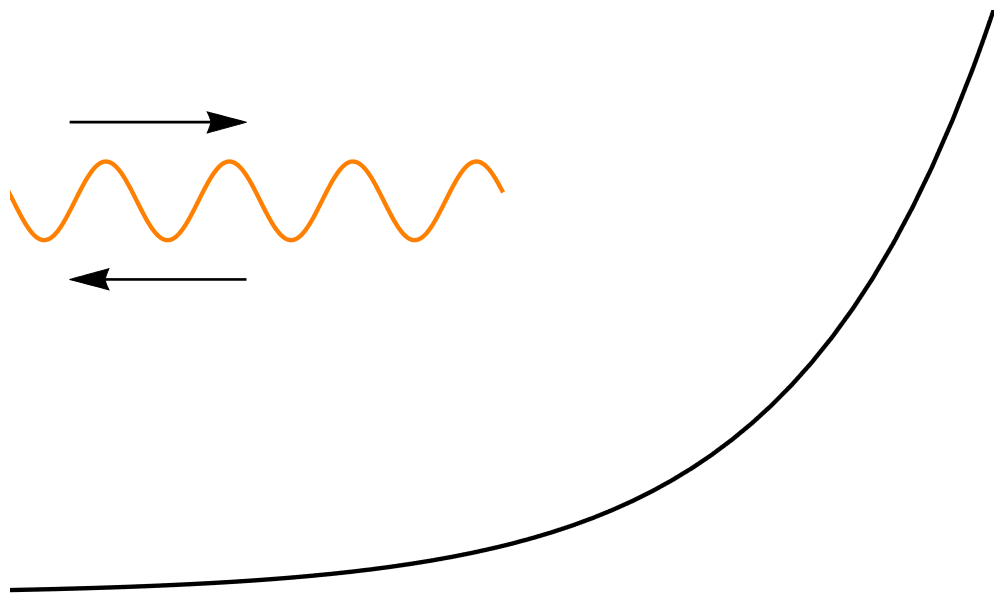
\includegraphics[width=0.85\textwidth]{figures/fig08.png}
  \caption{Liouville CFT 中的标量原初场描述场空间中偏离 Liouville 墙的散射态。（原文 p.19，图 8）}
  \label{fig:8}
\end{figure}

特别地，零模 $\phi_0(\tau)$ 受到势 $V(\phi_0)=2\pi\mu e^{2b\phi_0}$ 的作用。若忽略 $n\neq0$ 的振子 $\phi_n$——在 $\phi_0\to-\infty$ 区域，对最低激发态而言这个近似可以成立——则能量本征态是由如下渐近波函数描述的散射态
\begin{equation}
  \label{eq:3-68}
  \Psi_P(\phi_0)\sim S(P)^{-\frac{1}{2}}e^{2iP\phi_0}+S(P)^{\frac{1}{2}}e^{-2iP\phi_0},
\end{equation}
其能量为
\begin{equation}
  \label{eq:3-69}
  h+\tilde h-\frac{c}{12}=2P^2.
\end{equation}
这些就是柱面上对应原初场 $V_P$ 的态。
% [Tutor Note: 按 p.18 的约定 $c=1+6Q^2$、$h=\frac{Q^2}{4}+P^2$ 直接代入，应有 $h+\tilde h-\frac{c}{12}=2P^2-\frac{1}{12}$；原文 (3.69) 少了 $-\frac{1}{12}$，也可能是作者把柱面能量零点另行约定，引用此式时须核对。]

\section{已知二维 CFT 概览}\label{sec:4}

\begin{keytakeaways}
  \item 核心物理图像：二维 CFT 有几类基本构造——自由玻色子的手征与反手征分量、离散对称群的轨形、流代数的 WZW 模型与陪集，以及非线性 sigma 模型。它们共同的约束是 OPE 的单值性与结合性、幺正性，以及环面上的模不变性。
  \item 使用的数学工具：偶自对偶格（Narain 格）、共轭类与扭曲扇区、拓扑线算符、仿射李代数及其 Sugawara 构造、顶点算符代数与模矩阵 $S,T$、$\beta$ 函数与 Ricci 流。
  \item 本节结论：模不变性把 Narain 格的动量格限制为偶自对偶格；轨形的扭曲扇区谱由扭曲环面配分函数 $Z^g_h$ 决定；WZW 模型的中心荷为 $c^G=k\dim G/(k+h)$；RCFT 的谱只含有限多个表示且 $S^2=(ST)^3=\mathbb{I}$，故中心荷必为有理数；NLSM 的共形不变性等价于 $\beta^G_{ij}=\beta^\Phi=0$，即靶空间度规满足运动方程。
\end{keytakeaways}

下面我们简要回顾二维中一些已知的幺正 CFT 的构造。

\subsection{Narain 格}\label{sec:4-1}

一族基本的 CFT 由自由玻色子的全纯分量与反全纯分量构造，它们可由如下 OPE 定义：
\begin{equation}
  \label{eq:4-1}
  X_L^i(z)X_L^j(0)\sim-\delta^{ij}\ln z,\qquad X_R^i(\bar z)X_R^j(0)\sim-\delta^{ij}\ln\bar z .
\end{equation}
当然，这些场并非单值；思路是用它们构造出满足单值、结合 OPE 的算符，并且要求算符谱同时模不变。

% [Tutor Note: (4.1) 的系数 $-\delta^{ij}$ 与两点函数 $\langle X(z)X(0)\rangle=-\ln|z|^2$ 的约定一致。若采用带 $\alpha'$ 的约定 $X^iX^j\sim-\frac{\alpha'}{2}\delta^{ij}\ln z$，则 (4.3) 的顶点算符要相应乘 $\sqrt{2/\alpha'}$，(4.4) 的整内积条件也会随之改动；比较不同文献时须先确认此项归一化。]

我们先取一组 $U(1)^{n_L}$ 全纯流与 $U(1)^{n_R}$ 反全纯流，
\begin{equation}
  \label{eq:4-2}
  j^i(z)=\partial X_L^i(z),\qquad \tilde j^i(\bar z)=\bar\partial X_R^i(\bar z).
\end{equation}

接下来考虑如下形式的流代数原初场
\begin{equation}
  \label{eq:4-3}
  V_{k_L,k_R}=\,:e^{ik_L\cdot X_L+ik_R\cdot X_R}:,
\end{equation}
其中 $k=(k_L,k_R)$ 视为 $\mathbb{R}^{n,m}$ 中的矢量。OPE 的自洽性要求 $k$ 取值于一个内积为整数的格 $\Gamma\subset\mathbb{R}^{n,m}$：
\begin{equation}
  \label{eq:4-4}
  k\circ k'\equiv k_L\cdot k'_L-k_R\cdot k'_R\in\mathbb{Z}.
\end{equation}
模不变性进一步要求 $\Gamma$ 是偶格且自对偶 \cite{r18}。设 $e_a$ 为 $\Gamma$ 的一组基，则 $A_{ab}\equiv e_a\circ e_b$ 是偶幺模矩阵。这样的格必须满足 $n-m\equiv0\pmod 8$。若 $n,m\ge1$，即 $\Gamma$ 为不定号，比如 $n-m=8k$、$k,m\ge1$，则在格同构意义下 $\Gamma$ 等价于 $\Gamma_8^{\oplus k}\oplus\Gamma_{1,1}^{\oplus m}$；其中 $\Gamma_8$ 是 $E_8$ 的根格，$\Gamma_{1,1}$ 是号差为 $(1,1)$、配对矩阵由 Pauli 矩阵 $\sigma_1$ 给出的格。对于秩 $n=8k$ 的正定号偶自对偶格，$k=1$ 时 $\Gamma_8$ 是唯一的选择，$k=2$ 时有两个不等价的格：$\Gamma_8\oplus\Gamma_8$ 与 $\Gamma_{16}$。

% [Tutor Note: 此处 "$A_{ab}$ 为偶幺模矩阵" 与 "$n-m\equiv0\pmod 8$" 是两条独立条件：幺模指 $\det A=\pm1$，偶指对角元 $e_a\circ e_a\in2\mathbb{Z}$。"秩为 8 的倍数"来自偶幺模格的 Milgram 定理；而 $n-m=8k$ 时不定号格由 $\Gamma_8^{\oplus k}\oplus\Gamma_{1,1}^{\oplus m}$ 唯一决定；正定号情形在秩 8、16 时分别只有 $\Gamma_8$ 与 $\Gamma_{16}=\Gamma_8^{\oplus2}$，但秩 24 有 24 个 Niemeier 格，故 $k\ge3$ 时并不唯一。这是 Narain 模空间讨论的起点。]

\subsection{轨形}\label{sec:4-2}

若一个 CFT 具有离散对称群 $G$，通常可以规范（gauge）这个 $G$（但并非总能如此，原因在于 't Hooft 反常）。这种构造称为轨形 \cite{r19}。轨形 CFT 的局域算符希尔伯特空间（或柱面上的态空间）形如
\begin{equation}
  \label{eq:4-5}
  \mathcal{H}=\bigoplus_{[g]}\mathcal{H}_{[g]},
\end{equation}
其中求和遍历 $G$ 的共轭类。特别地，$\mathcal{H}_{[1]}$ 是原 CFT 中 $G$ 不变的态空间，称为未扭曲扇区；其余的 $\mathcal{H}_{[g]}$ 称为扭曲扇区。

扭曲扇区可以形式地如下构造。对于黎曼面 $\Sigma$ 上的 CFT 与给定的元素 $g\in G$，可以定义一个线算符 $L_g$：它沿环绕 $\Sigma$ 某个把手的定向回路放置，使得穿过该把手、分居 $L_g$ 两侧传播的态相差 $g$ 的对称作用。由于 $G$ 是对称性，线算符 $L_g$ 是拓扑的，即可以在不改变 $\Sigma$ 上 CFT 的配分函数或关联函数的前提下连续形变（允许劈裂与合并）。若干线算符 $L_{g_i}$（$i=1,\cdots,n$）可按循环次序在一点相遇，条件是 $g_1\cdots g_n=1$。特别地，当 $g$ 与 $h$ 对易时，$L_g$ 与 $L_h$ 可以相交。

设 $g,h$ 是 $G$ 中一对对易元素，记 $Z^h_g$ 为原 CFT 在空间圈上插入线算符 $L_g$、在欧几里得时间圈上插入线算符 $L'_h$ 时的环面配分函数。轨形 CFT 的扭曲扇区 $\mathcal{H}_{[g]}$ 的配分函数满足
\begin{equation}
  \label{eq:4-6}
  \operatorname{Tr}_{\mathcal{H}_{[g]}}q^{L_0-\frac{c}{24}}\bar q^{\bar L_0-\frac{\bar c}{24}}=\frac{1}{|C_g|}\sum_{h\in C_g}Z^h_g,
\end{equation}
其中 $C_g$ 是 $g$ 在 $G$ 中的交换子（中心化子）。

% [Tutor Note: (4.6) 左边是对 $\mathcal{H}_{[g]}$ 的迹，右边却对 $C_g$ 求和并除以 $|C_g|$，这正是在 $g$ 的交换子群上做有限群平均投影。只有与 $g$ 对易的 $h$ 才能同时在空间圈与时间圈上插入线算符，故 $Z^h_g$ 只在 $h\in C_g$ 时有定义；$\mathbb{Z}_2$ 轨形时 $|C_g|=|G|$，退化为通常的 $g$ 投影。]

一般而言，扭曲扇区的谱可由 $Z^1_g(\tau,\bar\tau)=Z^g_1(-1/\tau,-1/\bar\tau)$ 确定。类似地，可以确定一个未扭曲算符与一对 $g$、$g^{-1}$ 扭曲算符之间的三点函数。利用 $g_1,g_2,g_2^{-1},g_1^{-1}$ 扭曲扇区算符四点函数的 $s$ 道与 $t$ 道之间的交叉对称性，可以提取 $(g_1,g_2,g_2^{-1}g_1^{-1})$ 扭曲算符的结构常数。这是图~\ref{fig:9} 所示关系的一个特例。再转到 $u$ 道，考虑 $g_2$ 与 $g_2^{-1}$ 扭曲算符 OPE 中的单位道，就能得到 $g_1$ 扭曲扇区的 $g_2$ 扭曲环面特征标，即 $Z^{g_2}_{g_1}$，如图~\ref{fig:10} 所示。通过这一程序，轨形 CFT 的所有关联函数原则上都可以无歧义地确定。

\begin{figure}[htbp]
  \centering
  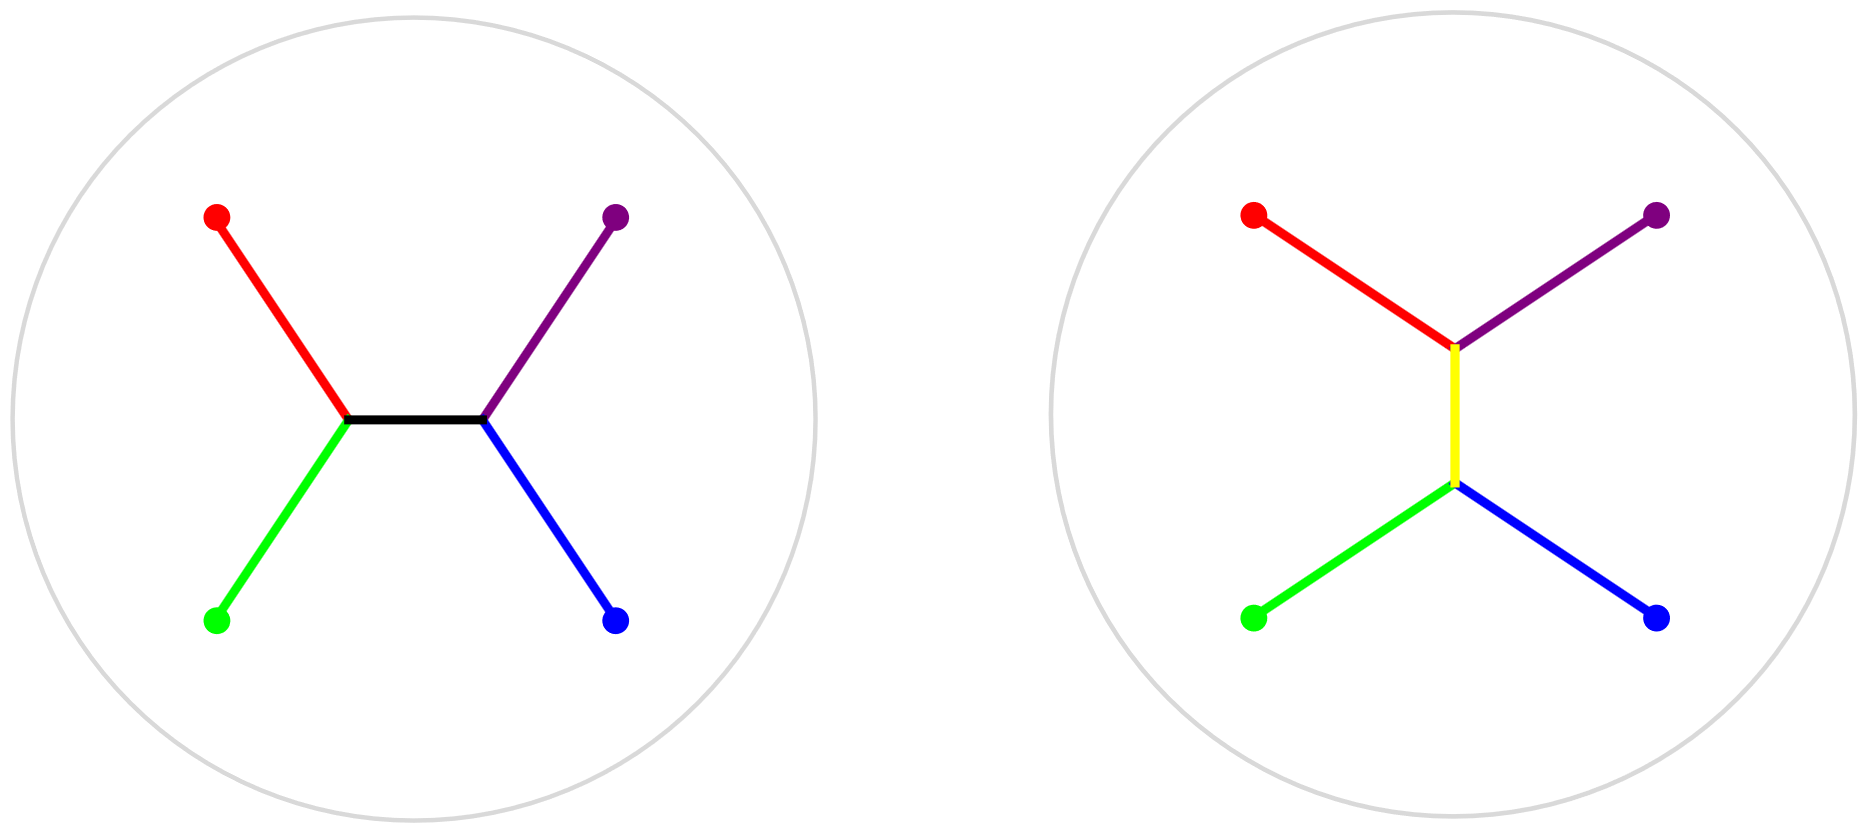
\includegraphics[width=0.85\textwidth]{figures/fig09.png}
  \caption{扭曲扇区算符 $\langle\phi_{g_1}\phi_{g_2}\phi_{g_3}\phi_{g_4}\rangle$ 的球面四点函数，由满足 $g_1g_2g_3g_4=1$ 的拓扑线算符连接。$s$ 道共形块分解涉及结构常数 $C_{g_1,g_2,(g_1g_2)^{-1}}C_{g_3,g_4,g_1g_2}$，而 $t$ 道涉及 $C_{g_2,g_3,(g_2g_3)^{-1}}C_{g_4,g_1,g_2g_3}$（记号只是示意性的，因为我们只用扭曲扇区标记了结构常数中的原初场）。（原文 p.21，图 9）}
  \label{fig:9}
\end{figure}

\begin{figure}[htbp]
  \centering
  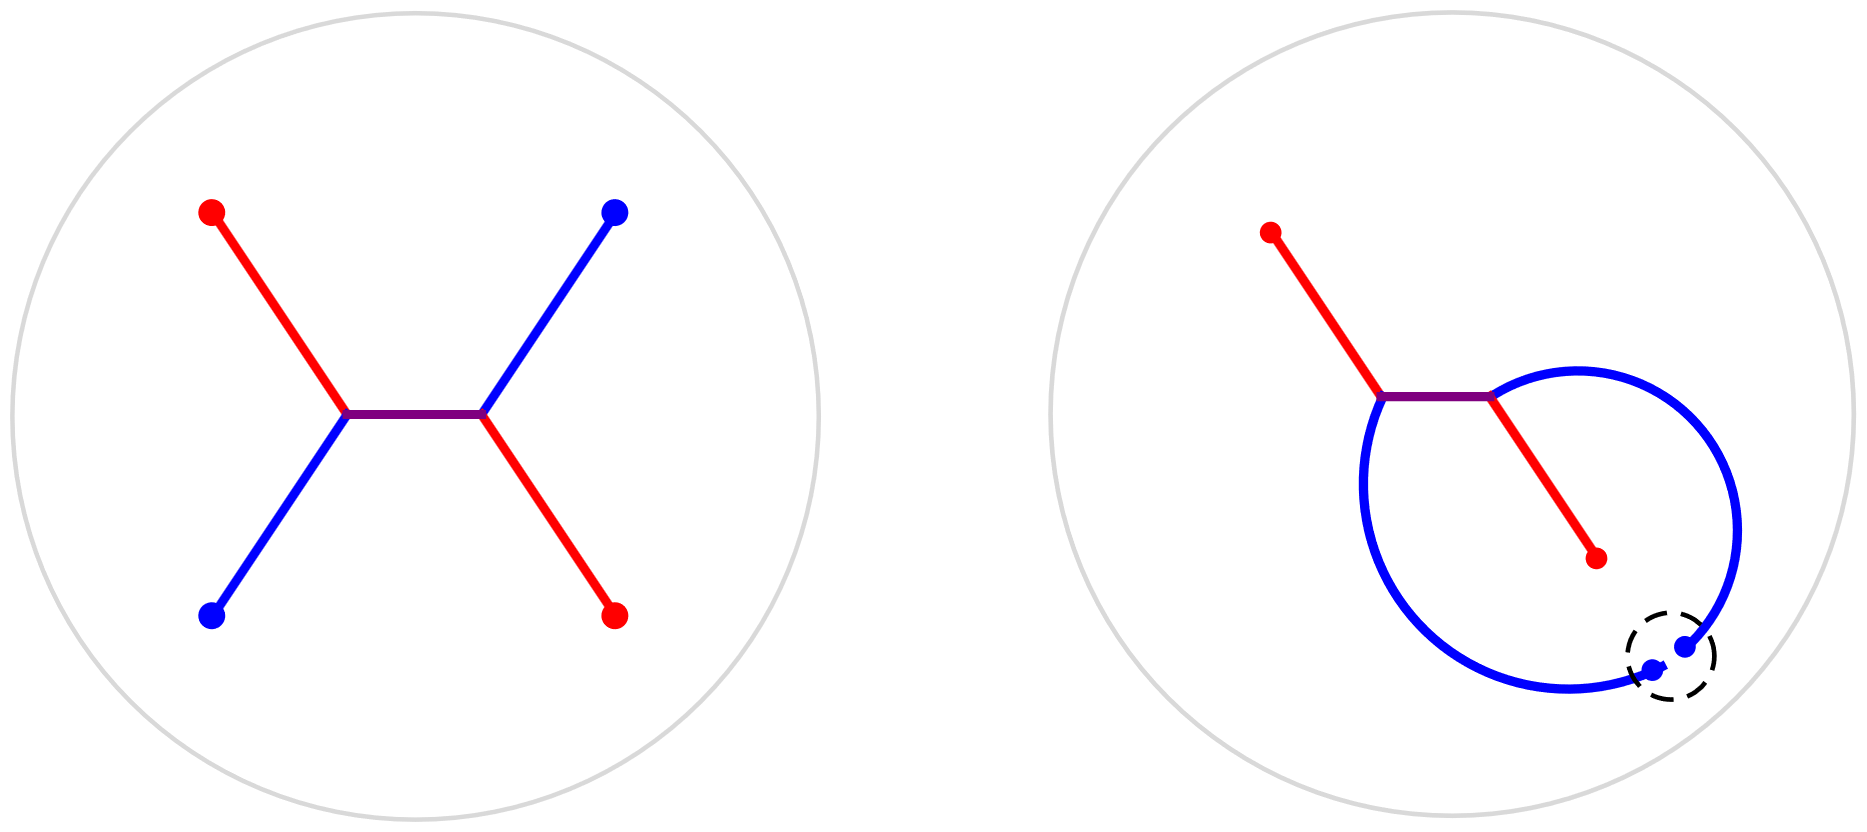
\includegraphics[width=0.85\textwidth]{figures/fig10.png}
  \caption{对于一对对易元素 $g,h$，$u$ 道 OPE 极限下的扭曲场关联函数 $\langle\phi_g\phi_h\phi_{g^{-1}}\phi_{h^{-1}}\rangle$ 决定了最一般的扭曲环面特征标 $Z^g_h$。（原文 p.21，图 10）}
  \label{fig:10}
\end{figure}

作为一个非平凡的实例，考虑基于 Leech 格 $L_{24}$ 的、$c=24$、$\bar c=0$ 的 Narain 格 CFT。$L_{24}$ 是号差为 $(24,0)$ 的偶自对偶格，其特殊性质是不含长度平方等于 $2$ 的格矢量。$L_{24}$ CFT 的环面配分函数为
\begin{equation}
  \label{eq:4-7}
  Z(\tau)=j(\tau)-720,
\end{equation}
其中 $j(\tau)$ 是椭圆 $j$ 不变量
\begin{equation}
  \label{eq:4-8}
  j(\tau)=\frac{E_4(\tau)^3}{\eta(\tau)^{24}}=q^{-1}+744+196884q+21493760q^2+\cdots.
\end{equation}

考虑 $L_{24}$ 的 $\mathbb{Z}_2$ 对称性，其生成元 $g$ 的作用是对所有格元素取反射，即把 24 个手征玻色子全部反射 $X^i_L\to-X^i_L$。相应的环面特征标为
\begin{equation}
  \label{eq:4-9}
  Z^g_1(\tau)=q^{-1}\prod_{n=1}^{\infty}\frac{1}{(1+q^n)^{24}}=\left[\frac{2\eta(\tau)}{\theta_2(\tau)}\right]^{12}.
\end{equation}

% [Tutor Note: (4.9) 的 $\theta$ 函数恒等式可逐步验证：$\theta_2(\tau)=2q^{1/8}\prod_{n\ge1}(1-q^n)(1+q^n)^2$，$\eta(\tau)=q^{1/24}\prod_{n\ge1}(1-q^n)$，故 $\frac{2\eta}{\theta_2}=q^{-1/12}\prod_{n\ge1}(1+q^n)^{-2}$，取 12 次方即得 $q^{-1}\prod_{n\ge1}(1+q^n)^{-24}$。在 $\tau\to-1/\tau$ 下 $\eta\to(-i\tau)^{1/2}\eta$、$\theta_2\to(-i\tau)^{1/2}\theta_4$，比值把 $\theta_2$ 换成 $\theta_4$，于是得到 (4.10)。]

其模 $S$ 变换为
\begin{equation}
  \label{eq:4-10}
  Z^1_g(\tau)=Z^g_1(-1/\tau)=\left[\frac{2\eta(\tau)}{\theta_4(\tau)}\right]^{12}.
\end{equation}
于是轨形 CFT $L_{24}/\mathbb{Z}_2$ 的环面配分函数为
\begin{equation}
  \label{eq:4-11}
  \begin{aligned}
  Z_{L_{24}/\mathbb{Z}_2}(\tau)&=\frac{1}{2}\left[Z^1_1(\tau)+Z^g_1(\tau)+Z^1_g(\tau)+Z^g_g(\tau)\right]\\
  &=\frac{1}{2}j(\tau)-360+2^{11}\bigl(\eta(\tau)\bigr)^{12}\left[\frac{1}{(\theta_2(\tau))^{12}}+\frac{1}{(\theta_4(\tau))^{12}}-\frac{1}{(\theta_3(\tau))^{12}}\right]\\
  &=j(\tau)-744.
  \end{aligned}
\end{equation}

% [Tutor Note: (4.7) 减去 $720$ 而不是 $744$，正是为了抵消 $j$ 的常数项 $744$：$L_{24}$ CFT 的配分函数常数项于是为 $24$，对应 24 个守恒流 $\partial X^i_L$；而 (4.11) 中四项按 $\frac{1}{2}j-360$ 与 $\theta$ 函数组合相加后恰消去常数项，故轨形后无自旋 1 流，这正是下一段所说的“$q^0$ 阶项不出现”。]

特别地，$q^0$ 阶项不出现，说明这个 CFT 中没有守恒的自旋 1 流。$L_{24}/\mathbb{Z}_2$ 轨形实际上具有很大的离散对称群，它同构于最大的散在单群，即 monster 群。这个 CFT 由 Frenkel、Lepowsky 与 Meurman 发现 \cite{r20}，因此也称为 monster CFT。

注意，给定一个 $n$ 阶元素 $g$，我们期望 $Z^1_g(\tau)=Z^g_1(-1/\tau)$ 在 $\tau\to\tau+n$ 下不变。若不成立，则由 $g$ 生成的 $\mathbb{Z}_n$ 所做的轨形就无法自洽地构造。这是离散 't Hooft 反常的一个例子。例如 monster 群有 194 个共轭类，其中 56 个因这类反常不能用来构造轨形。

% [Tutor Note: 这里 $Z^1_g(\tau)=Z^g_1(-1/\tau)$ 是做过 $S$ 变换后的量；若 $g$ 的阶为 $n$，则要求它在 $\tau\to\tau+n$（而不是 $\tau\to\tau+1$）下不变。这正是 $\mathbb{Z}_n$ 轨形自洽的模不变性条件，等价于该对称性没有离散 't Hooft 反常；monster 群的 194 个共轭类中有 56 个不满足，故不能用相应共轭类做轨形。]

\subsection{WZW 与陪集模型}\label{sec:4-3}

一个具有连续对称群 $G$ 的幺正二维 CFT 应当含有一组守恒的 Noether 流 $j^a_\mu$，它们作为局域原初算符出现，$a=1,\cdots,\dim G$。在紧致 CFT 中，这些流必然由权为 $(1,0)$ 的全纯算符 $j^a(z)$ 与权为 $(0,1)$ 的反全纯算符 $\tilde j^a(\bar z)$ 给出。此外，它们的 OPE 必须取流代数的形式；以全纯情形为例，
\begin{equation}
  \label{eq:4-12}
  j^a(z)j^b(0)\sim\frac{\kappa^{ab}}{z^2}+\frac{if^{ab}{}_c\,j^c(0)}{z}.
\end{equation}
这里 $f^{ab}{}_c$ 是 $G$ 的李代数结构常数，$\kappa^{ab}$ 正比于李代数上的一个不变双线性型。幺正性要求 $\kappa^{ab}$ 正定，这意味着 $G$ 半单且紧致。若 $G$ 是单紧致李群，可以写 $\kappa^{ab}=kd^{ab}$，其中 $d^{ab}$ 的逆 $d_{ab}$ 归一化为：对长根 $\psi$ 有 $\psi^2\equiv d_{ab}\psi^a\psi^b=2$。

记 $\hat G_k$ 为单李群 $G$ 的能级 $k$ 流代数。可以定义一个守恒的自旋 2 原初算符，即 Sugawara 能动张量 $T^G$：
\begin{equation}
  \label{eq:4-13}
  T^G(z)=\frac{1}{2(k+h)}\lim_{w\to z}\left[d_{ab}j^a(w)j^a(z)-\frac{k\dim G}{(w-z)^2}\right],
\end{equation}
% [Tutor Note: (4.13) 的被积项写作 $d_{ab}j^a(w)j^a(z)$，第二个流的指标又标成了 $a$。由于 $d_{ab}$ 需要缩并一对指标 $a,b$，这里应为 $d_{ab}j^a(w)j^b(z)$；原文照排，疑为笔误。另外 $2(k+h)$ 中的 $h$ 是下一段才定义的对偶 Coxeter 数，这个整体归一化因子保证 $T^G$ 的 OPE 给出中心荷 (4.14)。]

其中 $h$ 是对偶 Coxeter 数，由关系 $-f^{ac}{}_d f^{bd}{}_c=2h d^{ab}$ 定义。$T^G$ 的归一化使得 $T^G(z)T^G(0)$ 的 OPE 与能动张量的形式相同，其中心荷为
\begin{equation}
  \label{eq:4-14}
  c^G=\frac{k\dim G}{k+h}.
\end{equation}
CFT 能动张量的中心荷 $c$ 大于或等于 $c^G$。若 $c$ 恰等于 $c^G$，则 $T^G$ 也就等于 CFT 的能动张量 $T(z)$。

确实可以构造一个完全自洽的 CFT，其全纯与反全纯能动张量分别为 $T^G(z)$ 与 $\bar T^G(\bar z)$，这就是 Wess–Zumino–Witten（WZW）模型 \cite{r21,r22}。为此需要构造局域算符的谱；这些算符现在不仅可以按 Virasoro 代数的表示来组织，还可以按更大的流代数的表示来组织（因为 Virasoro 生成元可以由流构造出来）。流代数 $\hat G_k$ 的每个不可约表示由一个最低权流代数原初场集合 $\phi_i$ 生成，$\phi_i$ 在 $G$ 的不可约表示 $R$ 中变换，其 OPE 为
\begin{equation}
  \label{eq:4-15}
  j^a(z)\phi_i(0)\sim\frac{t^a_{ij}}{z}\phi_j(0).
\end{equation}
$\hat G_k$ WZW 模型恰好含有一组原初场 $\phi_{i\bar i}(z,\bar z)$，它们与左右流代数群 $G$ 的一对相同表示 $(R,R)$ 相联系；其中 $R$ 遍历 $G$ 的所有不可约表示，其最高权矢量 $\lambda$ 满足 $\langle\lambda,\theta\rangle\le k$，而 $\theta$ 是 $G$ 的最高根矢量。对 $G=SU(2)$，表示 $R$ 由自旋 $j$ 标记，该条件即 $j\le k/2$。

% [Tutor Note: $\langle\lambda,\theta\rangle\le k$ 中的 $\theta$ 取最高根，这一条件把 $\hat G_k$ 的表示限制为可积表示（最高权落在仿射 Weyl 群的 basic alcove 内），从而只留下有限多个幺正表示。对 $SU(2)_k$，自旋 $j$ 的最高权满足 $\langle\lambda,\theta\rangle=2j$，故条件化为 $2j\le k$，即 $j\le k/2$；同一条件用极小模型主场的 Kac 指标写就是 $1\le 2j+1\le k+1$。]

现在给定一个具有连续对称群 $H$、由流代数 $\hat H$ 支配的 CFT，可以尝试规范 $H$ 以得到新的 CFT。把 $\hat G$ WZW 模型的子群 $H\subset G$ 规范化，就得到所谓的 $G/H$ 陪集模型 \cite{r23,r24}。陪集模型完整算符谱的构造相当繁复，这里不详细讨论。注意有一族特殊的陪集模型 $(SU(2)_k\times SU(2)_1)/SU(2)_{k+1}$，它等价于 $A_k$ 极小模型，其中心荷为 $c=1-\frac{6}{(k+2)(k+3)}$。

% [Tutor Note: coset 模型的中心荷按 $c(G_k)-c(H_k)$ 计算；利用 $c(SU(2)_k)=3k/(k+2)$，有 $c=\frac{3k}{k+2}+1-\frac{3(k+1)}{k+3}=1-\frac{6}{(k+2)(k+3)}$，其中 $1=c(SU(2)_1)$ 这一项最容易漏掉。此式与 $A_k$ 极小模型的中心荷公式一致，说明同一 RCFT 可以有多种构造描述。]

\subsection{有理共形场论}\label{sec:4-4}

若一个幺正 CFT 在 Virasoro 代数之外还含有守恒的自旋 $s$ 流，则这些流必然是权为 $(s,0)$ 的全纯流或权为 $(0,s)$ 的反全纯流。先只看全纯算符。全纯算符的 OPE 自行闭合，给出一个扩充 Virasoro 代数的全纯（即手征）顶点算符代数，其一般形式为
\begin{equation}
  \label{eq:4-16}
  \mathcal{O}_a(z)\mathcal{O}_b(0)=\sum_c A_{ab}{}^c z^{-h_a-h_b+h_c}\mathcal{O}_c(0),
\end{equation}
其中 $h_a$ 是非负整数。全纯算符 $\mathcal{O}_a(z)$ 与一个权为 $(h,\tilde h)$ 的一般算符 $\phi$ 的 OPE 只能含有权为 $(h+n,\tilde h)$ 的算符，$n$ 为整数。因此，反全纯权为 $\tilde h$ 的算符集合构成全纯顶点算符代数的一个表示，该表示未必不可约。同样，全纯权为 $h$ 的算符集合构成反全纯顶点代数的一个表示。于是 CFT 的算符谱可以分解为全纯顶点算符代数的表示 $R_i$ 与反全纯顶点代数的表示 $\bar R_{\bar j}$。

$R_i$ 的环面特征标定义为
\begin{equation}
  \label{eq:4-17}
  \chi_i(\tau)=\operatorname{Tr}_{R_i}q^{L_0-\frac{c}{24}},
\end{equation}
类似地有 $\bar R_{\bar i}$ 的特征标 $\bar\chi_{\bar i}(\bar\tau)$。CFT 的环面配分函数可以写成
\begin{equation}
  \label{eq:4-18}
  Z(\tau,\bar\tau)=\sum_{i,\bar i}n_{i\bar i}\,\chi_i(\tau)\bar\chi_{\bar i}(\bar\tau),
\end{equation}
其中 $n_{i\bar i}$ 是非负整数简并度。有理共形场论（RCFT）是指谱中只含有限多个全纯与反全纯顶点算符代数表示的 CFT，即 \eqref{eq:4-18} 是有限和。此时 OPE 的闭合性要求所有权 $(h,\tilde h)$ 都是有理数。

在 $\tau\to\tau+1$ 下，有
\begin{equation}
  \label{eq:4-19}
  \chi_i(\tau+1)=T_{ij}\chi_j(\tau),\qquad T_{ij}=\delta_{ij}e^{2\pi i\left(h_i-\frac{c}{24}\right)}.
\end{equation}
同样有 $\bar\chi_{\bar i}(\bar\tau+1)=\tilde T_{\bar i\bar j}\bar\chi_{\bar j}(\bar\tau)$。环面配分函数的模不变性要求：只有当 $h_i-\tilde h_{\bar j}\in\mathbb{Z}$ 时 $n_{i\bar j}$ 才非零；并且在 $\tau\to-1/\tau$ 下，$\chi_i$ 变为自身的线性组合，$\bar\chi_{\bar i}$ 亦然：
\begin{equation}
  \label{eq:4-20}
  \chi_i(-1/\tau)=S_{ij}\chi_j(\tau),\qquad \bar\chi_{\bar i}(-1/\bar\tau)=\tilde S_{\bar i\bar j}\bar\chi_{\bar j}(\bar\tau),
\end{equation}
使得
\begin{equation}
  \label{eq:4-21}
  n_{i\bar i}S_{ij}\tilde S^*_{\bar i\bar j}=n_{j\bar j}.
\end{equation}

% [Tutor Note: (4.21) 中重复指标 $i,\bar i$ 按 Einstein 约定求和，等式两边的自由指标只剩 $j,\bar j$；它正是 $Z(\tau,\bar\tau)$ 在 $S$ 变换下不变的展开式，$\tilde S^*$ 上的复共轭来自 $\bar\chi$ 的复共轭。用 (4.18) 逐项代入即可得到此式。]

$T$ 与 $S$（以及类似地 $\tilde T$ 与 $\tilde S$）必须构成 $\mathrm{PSL}(2,\mathbb{Z})$ 的有限维表示，即
\begin{equation}
  \label{eq:4-22}
  S^2=(ST)^3=\mathbb{I}.
\end{equation}
这尤其意味着 $(\det S^2)^{-3}(\det(ST)^3)^2=\det T^6=1$，由此可知中心荷 $c$ 也必为有理数。

% [Tutor Note: 这个恒等式值得展开：由 $S^2=\mathbb{I}$ 得 $(\det S)^2=1$，由 $(ST)^3=\mathbb{I}$ 得 $(\det S\det T)^3=1$，于是 $(\det S^2)^{-3}(\det(ST)^3)^2=(\det S)^{-6}(\det S)^6(\det T)^6=\det T^6=1$。又 $\det T=\exp\left(2\pi i\sum_i\left(h_i-\frac{c}{24}\right)\right)$，故 $\sum_i h_i-\frac{nc}{24}\in\frac{1}{6}\mathbb{Z}$；结合 $h_i$ 的有理性即得 $c\in\mathbb{Q}$。]

RCFT 没有完整的分类，尽管所有已明确知道的例子都来自陪集模型或 Narain 格 CFT，及其乘积与轨形，并且位于其精确边缘形变的模空间的特殊点上。最简单的一类 RCFT 是亚纯 CFT（meromorphic CFT），其整个算符谱只由单个全纯顶点算符代数构成，例如前面讨论过的 $L_{24}$ CFT 及其 $\mathbb{Z}_2$ 轨形 monster CFT。即便是亚纯 CFT，也远未得到完整分类。

注意所有 $c>1$ 的 RCFT 都必须含有比 Virasoro 严格更大的全纯顶点算符代数，因为非退化的环面 Virasoro 特征标并不在 $\mathrm{PSL}(2,\mathbb{Z})$ 的有限维表示中变换。换句话说，所有 $c>1$ 的 RCFT 都含有超出 Virasoro 代数的高自旋对称性。

\subsection{非线性 sigma 模型（NLSM）}\label{sec:4-5}

由拉氏量
\begin{equation}
  \label{eq:4-23}
  S=\frac{1}{4\pi}\int d^2\sigma\,\sqrt{g}\,G_{ij}(X)g^{ab}\partial_a X^i\partial_b X^j
\end{equation}
定义的二维非线性 sigma 模型（NLSM）在经典意义上是 Weyl 不变的。若路径积分能以尊重共形对称性的方式正规化，它就会给出一个 CFT，但这远非必然。我们需要研究它的重整化群流：或者分析以 \eqref{eq:4-23} 为基础、配以适当正规化方案由路径积分定义的 1PI 量子有效作用量，或者分析包含所有可能的相关与边缘算符的 Wilson 有效作用量。Wilson 图像在这里相当模糊，因为微扰论中有无穷多个相关算符。其他经典边缘形变具有形式
\begin{equation}
  \label{eq:4-24}
  \frac{1}{4\pi}\int d^2\sigma\,B_{ij}(X)\epsilon^{ab}\partial_a X^i\partial_b X^j+\frac{1}{8\pi}\int d^2\sigma\,\sqrt{g}\,R^{(2)}\Phi(X).
\end{equation}
上式第一项，即 $B$ 场，是宇称奇的。它出现在 WZW 模型的拉氏量描述中：后者相当于群流形 $G$ 上带有非平凡 3-形式通量 $H=dB$ 的 NLSM。第二项涉及二维标量曲率；当 $X$ 为常数时它是拓扑项，在平坦二维时空中消失，其作用是修改能动张量，从而修改场 $X^i$ 的共形变换。这一项例如出现在陪集模型的 NLSM 描述中，最简单的非平凡例子是 $SU(2)/U(1)$ 模型，以及等价于 $SL(2)/U(1)$ 陪集模型的“cigar CFT”。

% [Tutor Note: (4.24) 第二项系数 $\frac{1}{8\pi}$ 与第一项的 $\frac{1}{4\pi}$ 相差因子 2，来源是 $\sqrt{g}R^{(2)}$ 的标准归一化；若改用 $\frac{1}{4\pi\alpha'}$ 的拉氏量约定，两式的相对系数会随之改变。当 $X$ 为常数时第二项化为 $\chi(\Sigma)\Phi$ 型的拓扑项（Gauss–Bonnet 定理），在环面（$\chi=0$）上确实消失；注意 $\chi=0$ 的是环面，而非任意平坦时空。]

至少在无 $B$ 场时，可以用维数正规化（形式上在 $d=2-\epsilon$ 维工作）直接正规化路径积分，并微扰地计算 1PI 有效作用量，或更直接地计算能动张量的迹：
\begin{equation}
  \label{eq:4-25}
  T^a{}_a=-\frac{\epsilon}{2}G_{ij}(X)\partial^a X^i\partial_a X^j+\frac{\epsilon}{4}R^{(2)}\Phi(X)-\frac{1}{2}\nabla_X^2\Phi(X).
\end{equation}
要把它变成量子理论中有意义的算符方程，需要把右边用重整化算符改写，然后取 $\epsilon\to0$ 极限。最终得到如下形式的算符方程：
\begin{equation}
  \label{eq:4-26}
  T^a{}_a=\frac{1}{2}\left[\beta^G_{ij}(X)\partial^a X^i\partial_a X^j\right]_r-\frac{1}{4}R^{(2)}\left[\beta^\Phi(X)\right]_r,
\end{equation}
其中 $[\cdots]_r$ 表示某种算符正规化，$\beta^G_{ij}$ 与 $\beta^\Phi$ 到前两个非平凡微扰阶为 \cite{r25}
\begin{equation}
  \label{eq:4-27}
  \begin{aligned}
  \beta^G_{ij}&=R_{ij}+\frac{1}{2}R_i{}^{k\ell m}R_{jk\ell m}+2\nabla_i\nabla_j\Phi+\cdots,\\
  \beta^\Phi&=-\nabla^2\Phi+(\nabla\Phi)^2+\frac{1}{4}R^{ijk\ell}R_{ijk\ell}+\cdots.
  \end{aligned}
\end{equation}

% [Tutor Note: (4.27) 中 $\frac{1}{2}R_i{}^{k\ell m}R_{jk\ell m}$ 是二圈引力 beta 函数的标志项，$\beta^\Phi$ 的一圈部分是 $-\nabla^2\Phi+(\nabla\Phi)^2$，二圈部分则是 $\frac{1}{4}R^{ijk\ell}R_{ijk\ell}$；若在 $\beta^G_{ij}$ 中把 $R_{ij}$ 也一并按“一圈+二圈”分组，则它分别对应量纲 2 与量纲 4 的算符。注意 $R_i{}^{k\ell m}$ 的第一个指标在上、其余在下，与 $R_{jk\ell m}$ 缩并后得到对称张量；指标位置摆错会差一个符号。]

共形不变性等价于条件 $\beta^G_{ij}=\beta^\Phi=0$。事实上，后者等价于基于有效作用量 $S_{\rm eff}[G_{ij}(X),\Phi(X)]$ 的靶空间运动方程。这些方程可以在靶空间局部求解，但解的整体存在性——尤其当靶空间紧致时——远非显然。
